%------------------------------------------------------------
%
\documentclass{article}
%
\usepackage[margin=2.5cm,tmargin=1cm,bmargin=1cm]{geometry}
\usepackage{amsmath}%
\usepackage{amsfonts}%
\usepackage{amssymb}%
%\usepackage{fullpage}
\usepackage{graphicx}
%\usepackage{setspace}
%\usepackage{float}
\usepackage{hyperref}
\usepackage{tikz}
\usepackage{xcolor}
\usepackage[normalem]{ulem}
\usepackage[outline]{contour}

\pagestyle{empty}
\newcommand{\firstDueDate}{Sept. 15}
\newcommand{\secondDueDate}{Oct. 1}
\newcommand{\thirdDueDate}{Oct. 15}
\newcommand{\fourthDueDate}{Nov. 1}
\newcommand{\fifthDueDate}{Nov. 15}
\newcommand{\methodsDueDate}{Nov. 15}
\newcommand{\finalDueDate}{Dec. 1}
\newcommand{\integrityLink}{\url{https://stedwards.app.box.com/s/izo4b4q9hywr5bfiq93ll4s8bls69rk1}}
\newcommand{\DSTstart}{Mar. 10}
\newcommand{\DSTend}{Nov. 3}




%\renewcommand*{\theenumi}{\thesection.\arabic{enumi}}
\newcommand{\BE}{\begin{equation}}
\newcommand{\EE}{\end{equation}}
\newcommand{\BEBA}{\begin{equation}\begin{aligned}}
\newcommand{\EAEE}{\end{aligned}\end{equation}}

\newcommand{\tikzcircle}{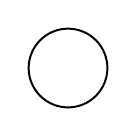
\begin{tikzpicture}\draw[black, line width=0.25mm] (0.5,0.5) circle (0.5); \end{tikzpicture}}
%tkzpiccntr: draw a picture centered at the given location
%usage: \tkzpiccntr{x,y}{width}{height}{filename}
\newcommand{\tkzpiccntr}[4]{\filldraw [fill=white](#1)++(-0.5*#2,-0.5*#3) rectangle +(#2,#3) [path picture=
	{
		\node at (path picture bounding box.center) 
		{
			\includegraphics[width=#2cm]{#4}
		};
	}
];
}

\newcommand{\tikzmoon}{\tkzpiccntr{0.5,0.5}{1}{1}{full_moon_white_bg.png};\draw[black, line width=0.25mm] (0.5,0.5) circle (0.5);}
\newcommand{\BP}{\begin{tikzpicture}}
\newcommand{\EP}{\end{tikzpicture}}

\newcommand{\tikzmoonNew}{\BP\draw[black, line width=0.25mm] (0,0) -- (1,0) -- (1,1) -- (0,1) -- cycle;\fill[black] (0.5,0.5) circle(0.5);\EP}
\newcommand{\tikzmoonWxC}{\BP\tikzmoon\fill[black] (0.5,0.0) arc(270:90:0.5) arc (90:-90:0.25 and 0.5) -- cycle;\EP}
\newcommand{\tikzmoonFQ}{\BP\tikzmoon\fill[black] (0.5,0.0) arc(270:90:0.5) -- cycle;\EP}
\newcommand{\tikzmoonWxG}{\BP\tikzmoon\fill[black] (0.5,0.0) arc(270:90:0.5) arc (90:270:0.25 and 0.5) -- cycle;\EP}
\newcommand{\tikzmoonFull}{\BP\tikzmoon;\EP}
\newcommand{\tikzmoonWnG}{\BP\tikzmoon\fill[black] (0.5,0.0) arc(-90:90:0.5) arc (90:-90:0.25 and 0.5) -- cycle;\EP}
\newcommand{\tikzmoonTQ}{\BP\tikzmoon\fill[black] (0.5,0.0) arc(-90:90:0.5) -- cycle;\EP}
\newcommand{\tikzmoonWnC}{\BP\tikzmoon\fill[black] (0.5,0.0) arc(-90:90:0.5) arc (90:270:0.25 and 0.5) -- cycle;\EP}


\begin{document}
\begin{center}\textbf{Moon Project Observations}\end{center}
Name : \underline{\hphantom{XXXXXXXXXXXXXXXXXXXXXXXX}}\hfill Fist Size: \underline{\hphantom{XXXXXX}}~Degrees\\
For each observation, note the date, time, \# of fists, and sketch the moon. See next page for details.

\begin{center}
\begin{tabular}{|c|c|c|c|c||c|c|c|c|}
\hline
\hphantom{XX}Date\hphantom{XX} & Clock Time & Moon        & Phase  & Fists   & Local Decimal & Solar & Moon  & Elongation\\
(mm/dd)                        & (24 hr)    & Sketch      & Number & (E or W)&  Time (h)     & HA (h)& HA (h)& (${}^\circ$)       \\
\hline
                               &            & \tikzcircle &        &         &                &      &       &           \\
\hline
                               &            & \tikzcircle &        &         &                &      &       &           \\
\hline
                               &            & \tikzcircle &        &         &                &      &       &           \\
\hline
                               &            & \tikzcircle &        &         &                &      &       &           \\
\hline
                               &            & \tikzcircle &        &         &                &      &       &           \\
\hline
                               &            & \tikzcircle &        &         &                &      &       &           \\
\hline
                               &            & \tikzcircle &        &         &                &      &       &           \\
\hline
                               &            & \tikzcircle &        &         &                &      &       &           \\
\hline
                               &            & \tikzcircle &        &         &                &      &       &           \\
\hline
                               &            & \tikzcircle &        &         &                &      &       &           \\
\hline
                               &            & \tikzcircle &        &         &                &      &       &           \\
\hline
                               &            & \tikzcircle &        &         &                &      &       &           \\
\hline
                               &            & \tikzcircle &        &         &                &      &       &           \\
\hline
                               &            & \tikzcircle &        &         &                &      &       &           \\
\hline
                               &            & \tikzcircle &        &         &                &      &       &           \\
\hline
                               &            & \tikzcircle &        &         &                &      &       &           \\
\hline
                               &            & \tikzcircle &        &         &                &      &       &           \\
\hline
                               &            & \tikzcircle &        &         &                &      &       &           \\
\hline
\end{tabular}
\end{center}
\newpage
\begin{center}\textbf{Moon Project Observation Instructions}\end{center}
\vspace{0.5cm}
\noindent For each observation, record the date, clock time, a sketch of the Moon, the phase number, and a measure of the Moon's hour angle. The remainder of the fields can be calculated at a later time. For the hour angle measurement, stand facing south (use the compass on your phone or a map to determine a known point that is directly south of you), then extand your arm directly in front of you (i.e. directly south). Raise your arm about 2/3 of the way to straight overhead (specifically, $60^\circ$). Close your both fists and one eye, then using alternating fists, count how many fists it takes to get to the Moon from the starting point. If the Moon is to the right of the starting point, it is west; if it is to the left, it is east. 

The Moon is often visible during the day, not just at night. Some observations will have to be made during the day.

\noindent
\begin{tabular}{p{1.25in}p{5in}}
\textbf{Date} & Enter the date (month and day) of the observation\\
\textbf{Clock time} & Enter the time at which you make the observation. Use 24~hr format, so 6:05~am is 06:05, 6:32~pm is 18:32, 12:15~am (shortly after midnight) is 00:15, and 12:15~pm (shortly after noon) is 12:15.\\
\textbf{Moon Sketch} & Pencil or ink in the portion of the Moon that is dark, leaving the illuminated portion of the Moon's disk as white. Then, lightly sketch notable features (if any) such as craters or maria (the darker parts of the moons surface). Pay close attention to which side is illuminated and more rounded.\\
\textbf{Phase Number} & Record a number that corresponds to the observed phase of the Moon. Use decimal numbers (i.e. 4.5, not just 4 or 5) when appropriate. The phase numbers are as follows:\\
\end{tabular}
\begin{tabular}{|l|cccccccc|}
\hline
\textit{Phase}	 &  & Waxing & First & Waxing &  & Waning & Third & Waning\\
\textit{Name} & New & Crescent & Quarter & Gibbous & Full & Gibbous & Quarter & Crescent\\
\textit{Sketch} & \tikzmoonNew& \tikzmoonWxC & \tikzmoonFQ & \tikzmoonWxG & \tikzmoonFull & \tikzmoonWnG & \tikzmoonTQ & \tikzmoonWnC\\
\textit{Phase Number} & 0 & 1 & 2 & 3 & 4 & 5 & 6 & 7\\
\hline
\end{tabular}\\
\begin{tabular}{p{1.50in}p{4.75in}}
\textbf{Fists} & The angle (in fists) relative to the meridian that you measure. Make sure to indicate whether the angle is east or west (left or right) of the meridian.\\
\textbf{Local Decimal Time} & Calculate the local decimal time as follows: Local decimal time = $\mathrm{Clock~Time~(h)} + (\mathrm{Clock~Time~(min)} \div 60) + \mathrm{DST~correction} - 0.50~h$. The \textit{DST correction} is -1~h from 2~am on \DSTstart~through 2~am on \DSTend, and 0~h the rest of the year (e.g. \DSTend~and later). Round the local decimal time to the nearest 0.01~h.\\
\textbf{Solar HA} & This is the hour angle of the Sun at the time of observation. To calculate this, subtract 12.00 from the \textit{Local Decimal Time} then multiply $15^\circ~\mathrm{h}^{-1}$. Round the answer to the nearest 1°.\\
\textbf{Moon HA} &To calculate the Moon's hour angle for the observation, convert fists to degrees based upon your fist size in degrees: Moon HA in degrees = $\mathrm{Fists} \times ({}^\circ / \mathrm{Fist})$. Observations of the Moon to be east of the meridian means a negative hour angle, west of the meridian means a positive hour angle. Round the answer to the nearest 1°.\\
\textbf{Elongation} &Elongation is the angle between the Sun and the Moon. To calculate the elongation: Elongation = (Sun~HA - Moon~HA). If the elongation is negative, add 360°. Round the answer to the nearest 1°.\\
\end{tabular}
\newpage
\begin{center}\textbf{Moon Project Observation Examples}\end{center}
\vspace{0.5cm}
\textit{\textbf{Example Observations}} (For these examples, 1 Fist = $10^\circ$)\\
\begin{tabular}{|c|c|c|c|c||c|c|c|c|}
\hline
\hphantom{XX}Date\hphantom{XX} & Clock Time & Moon        & Phase  & Fists   & Local Decimal & Solar & Moon  & Elongation\\
(mm/dd)                        & (24 hr)    & Sketch      & Number & (E or W)&  Time (h)     & HA (°)& HA (°)& (°)       \\
\hline
8 Mar 2019                     &  12:43     & \tikzmoonWxC &   0.5  &   2.5~E &  12.22          & 3&  -25  &  28         \\
\hline
26 Apr 2019                    &  8:28      & \tikzmoonTQ &   6.0  &   1.5~W &  6.97          & -75&  15  &  270         \\
\hline
16 May 2019                    &  21:40     & \tikzmoonWxG&  3.5   &   3.5~E &  20.17         &  123& -35 &  158         \\
\hline
5 June 2019                    &  20:10     & \tikzmoonWxC&  0.5   &  6.5~W  &  18.67         & 100 & 65  & 35          \\
\hline
\end{tabular}
The first observation is made on March 8 at 12:43~pm. The Moon is observed to be a waxing crescent (it is barely lit and the lit portion is to the right), and is observed to be 2.5 fists to the left of the meridian.

The 24~hr clock time is 12:43. March 8 is before daylight saving time, so the DST correction is 0. The local decimal time is $(12 + 48\div60 - 0.5) = 12.22$. The hour angle of the Sun is then $(12.22 - 12)\times15^\circ~\mathrm{h}^{-1} = 3^\circ$. The hour angle of the Moon is $(-2.5\times10^\circ) = -25^\circ$. Finally, the elongation of the Moon is $(3^\circ - (-25^\circ)) = 28^\circ$.

The second observation is made on April 26 at 8:28~am. The Moon is observed to be at third quarter (it is half-lit and the lit portion is to the left), and is observed to be 1.5 fists to the right of the meridian.

The 24~hr clock time is 08:28. April 26 is during daylight saving time, so the DST correction is -1. The local decimal time is $(8 + 28\div60 - 1 - 0.5) = 6.97$. The hour angle of the Sun is then $(6.97 - 12)\times15^\circ~\mathrm{h}^{-1} = -75^\circ$. The hour angle of the Moon is $(1.5\times10^\circ) = 15^\circ$. Finally, the elongation of the Moon is $(-75^\circ - 15^\circ) = -90^\circ$. Since this is negative, we add $-90^\circ + 360^\circ = 270^\circ$.

The third observation is made on May 16 at 9:40~pm. The Moon is observed to be a waxing gibbous (it is more than half-lit and the lit portion is to the right), and is observed to be 3.5 fists to the left of the meridian.

The 24~hr clock time is 21:40. May 16 is during daylight saving time, so the DST correction is -1. The local decimal time is $(21 + 40\div60 - 1 - 0.5) = 20.166667$. We round this to 20.17. The hour angle of the Sun is then $(20.17 - 12)\times15^\circ~\mathrm{h}^{-1} = 122.55^\circ$, which we then round to 123°. The hour angle of the Moon is $(-3.5\times10^\circ) = -35^\circ$. Finally, the elongation of the Moon is $(123^\circ - 35^\circ) = 158^\circ$.

The fourth observation is made on June 5 at 8:10~pm. The Moon is observed to be a waxing crescent (it is less than half-lit and the lit portion is to the right), and is observed to be 6.5 fists to the right of the meridian.

The 24~hr clock time is 20:10. June 5 is during daylight saving time, so the DST correction is -1. The local decimal time is $(20 + 10\div60 - 1 - 0.5) = 18.66667$. We round this to 18.67. The hour angle of the Sun is then $(18.67 - 12)\times15^\circ~\mathrm{h}^{-1} = 100^\circ$. The hour angle of the Moon is $(6.5\times10^\circ) = 65^\circ$. Finally, the elongation of the Moon is $(100^\circ - 65^\circ) = 35^\circ$.

\end{document}
